\documentclass[twocolumn]{article}
\usepackage[utf8]{inputenc}
\usepackage{graphicx}
\usepackage[backend=bibtex]{biblatex}
\usepackage{geometry}
\usepackage{subcaption}
\usepackage{colortbl}
\usepackage[dvipsnames]{xcolor}

\geometry{margin=0.75in}
\definecolor{lightgray}{rgb}{0.9,0.9,0.9}

\addbibresource{references.bib}

\title{Sign Language Recognition using Temporal Classification \\ Milestone Report}
\author{Hardie Cate (ccate)\\ Fahim Dalvi (fdalvi) \\ Zeshan Hussain (zeshanmh)}
\date{November 14, 2015}

\begin{document}

\maketitle

\section{Introduction}
In the US alone, there are approximately 900,000 deaf or mute people whose primary mode of conversation is sign language. 
For these people, communication with non-signers is a daily struggle, and they are often disadvantaged when it comes to finding a job, accessing health care, etc.
There are a few emerging technologies aimed at overcoming these communication barriers, but most existing solutions rely on cameras to translate sign language into vocal language.
While these solutions are promising, they require the deaf or mute person to carry the technology with him/her or for a proper environment to be set up for translation.

One alternative is to move the technology onto the person’s body.
Devices like the Myo armband available in the market today enable us to collect data about the position of the user's hands and fingers over time.
Since each sign is roughly a combination of gestures across time, we can use these technologies for sign language translation.
For our project, we utilize a dataset collected by a group at the University of South Wales, which contains parameters, such as hand position, hand rotation, and finger bend, for 95 unique signs.
For each input stream representing a sign, we predict which sign class this stream falls into.
We begin by implementing baseline SVM and logistic regression models, which perform reasonably well on high-quality data.
Lower quality data requires a more sophisticated approach, so we explore different methods in temporal classification, including long short-term memory architectures and sequential pattern mining methods. 

\section{Related Work}
Several techniques have been used to tackle the problem of sign language to natural language translation. Conventionally, sign language translation has involved taking an input of video sequences, extracting motion features that reflect sign language linguistic terms, and then using machine learning or pattern mining techniques on the training data. For example, Ong et al. propose a novel sequential pattern (SP) mining method that utilizes tree structures to classify signs \cite{ong2012sign}. Their data was captured using a mobile camera system and the motion features extracted included motion of the hands, location of the sign being performed, and handshapes used. These data are collected temporally (i.e. at multiple time steps). The authors use an SP method in order to address common issues with other models that have been used for sign language classification and translation, including unrefined feature selection and non-discriminatory learning. In general, there has been significant work done in using sequential pattern mining methods to analyze temporal data \cite{ong2012sign}\cite{papapetrou2007}.

Other techniques that do not involve visual input have also been studied. For example, Kadous uses a novel technique in his paper to improve classic machine learning algorithms by creating meta-features \cite{kadous2002temporal}. These meta-features are derived from the raw features by looking at important events in the time-series data. An example Kadous uses in his paper is the vertical maxima that a person's wrist reaches while signing. A meta-feature like this gives meaning to the "y-axis" in the data, and helps create better features. He also looks at other automatic techniques to generate these meta-features by looking for variations across time in a given dataset. Another study by Mehdi et al. proposes the use of neural networks to classify signs correctly \cite{mehdi2002sign}. They focus on signs that have distinct static shapes rather than analyzing the signs over time. Finally, a study by Graves et al. uses strong classification to predict a sequence of labels given time-series data, rather than a single label \cite{graves2006connectionist}. They use a recurrent neural network (RNN) integrated with a softmax classifier to achieve this prediction. 

\section{Datasets}
We are primarily using two datasets from the research project by Kadous \cite{kadous2002temporal}. The first dataset is a high quality dataset, with data recorded at a frequency of 200 Hz. This dataset was recorded using two 5 dimensional flock gloves on each hand. We have access to 6-bit precision finger bend measures for each finger, as well as 14-bit precision orientation and position of each wrist in space. The second dataset is a low quality dataset, with data available for only one hand. The data was recorded at a much lower frequency of 25 Hz using the Nintendo Powerglove. We only have 2-bit precision for the finger bend measures, and data was recorded for only 4 fingers. The position of the wrist also has a lower precision of 8-bits. In addition, we have access to only one degree of rotation, which was recorded at roughly 4-bit precision. Both datasets consists of time-series data for 95 signs. Each sign was repeated 27 times across various sessions. The source of the high quality data was a single professional signer, while the low quality data was recorded using several signers of varying levels of proficiencies. 

Further, we have a dataset that our team has collected using the Myo armband \cite{myo}. The armband provides 8 EMG signals from the user's forearm, along with the position and orientation of the forearm. These EMG signals correlate to the movement of the wrist and fingers. However, we currently only have data for a few signs, and are collecting more to improve our dataset.

\section{Technical Approach}
\begin{figure}
\centering
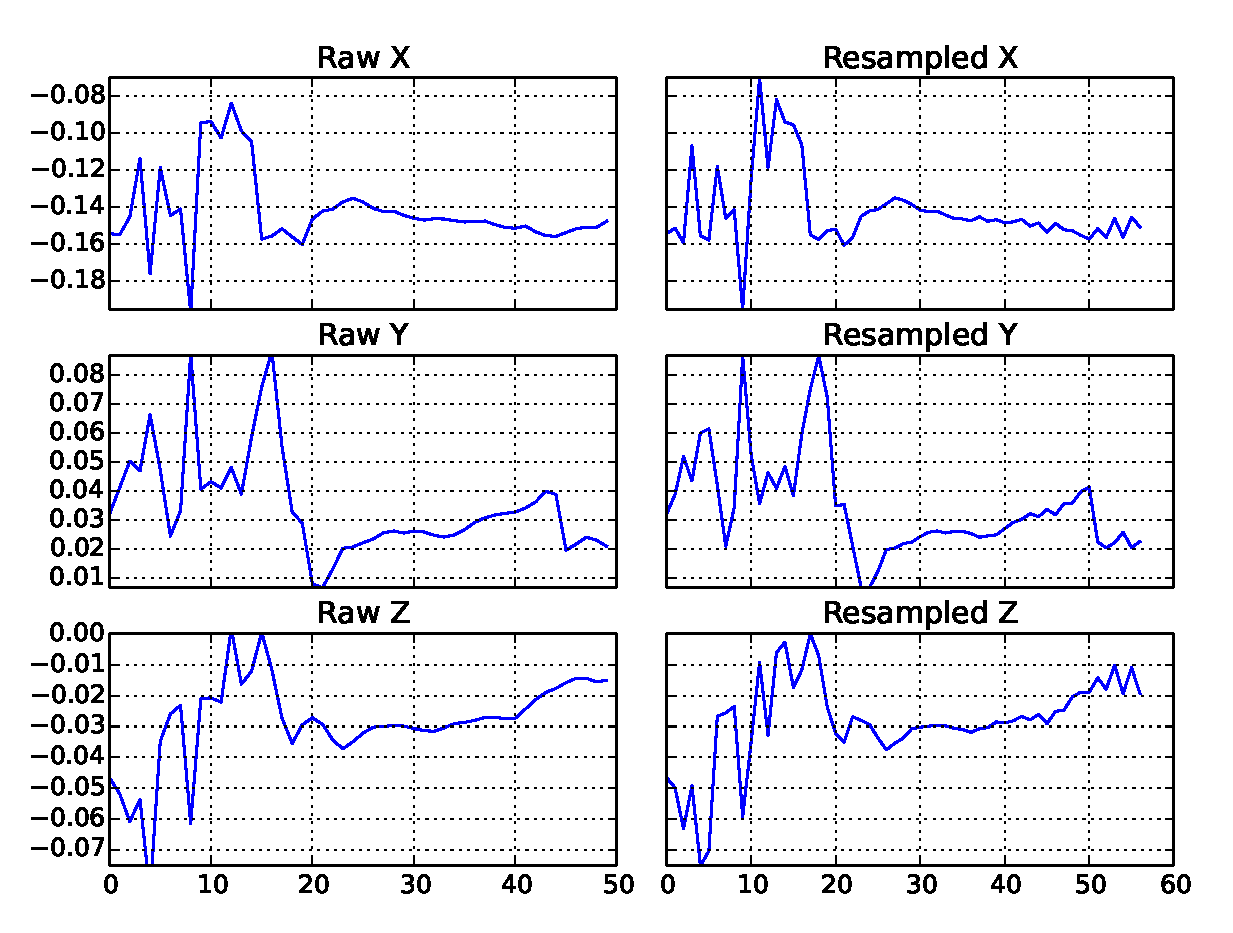
\includegraphics[width=\linewidth]{results/resampled_signal}
\caption{Signal resampling}
\label{fig:resample}
\end{figure}

We begin with several baseline implementations using SVM and logistic regression models.
The average number of frames for each sign is 57 frames, so we normalize all signs to this length by resampling using a fast Fourier transform. In Figure \ref{fig:resample}, the graphs on the left display readings for a single motion parameter over the lifetime of the sign, while the corresponding graphs on the right depict the resampled version. In general, we notice that there are not many differences between the original data and the resampled version. Most of the important information is retained, which supports our choice of normalization.

For our high quality dataset, each sample consists of a $22 \times 57$ matrix, where each row represents one of $22$ distinct motion parameters ($11$ for each hand) and each column is a particular frame. We process this data and store it in a 3-D matrix, whose dimensions are $2565 \times 22 \times 57$, where the first dimension is the number of examples, the second is the number features, and the third is the number of time frames.
In order to create an input matrix, $X$, that is ready for learning, we simply flatten the 3-D matrix so that the first 22 features are the reading at time $t=1$, the next 22 features correspond to time $t=2$, etc. Once we perform these preprocessing steps, we train SVM (with a linear kernel) and logistic regression models on our training set, which consists of 18 examples for each of the 95 signs. Then we train on the remaining 9 examples for each sign.

The next iteration of our approach will involve using other techniques such as sequential pattern mining and long short-term memory, which is a RNN architecture. For this report, we will focus on our LSTM approach. To address the concern that RNNs output a result at each frame, we will only consider the output after we have processed all the frames in the lifetime of a sign. Our architecture will model the form that was used by Graves et al. for speech recognition \cite{graves2013speech}. Specifically, in a regular recurrent neural network model, we compute an output vector sequence, $\mathbf{y}$, from an intermediate, hidden vector sequence, $\mathbf{h}$, and input vector sequence, $\mathbf{x}$. For the LSTM architecture, we will calculate $h_t$ at a specific time step via four sigmoid logistic functions, $i_t$, $f_t$, $c_t$ and $o_t$, commonly known as the input gate, forget gate, cell activator, and output gate.  

\section{Results}
\begin{table}[b]
    \centering
    \caption{Algorithm performance on the full dataset}
    \resizebox{\columnwidth}{!} {
        \begin{tabular}{|c|c|c|c|c|}
        \hline
         & SVM & Log. reg. & SVM & Log. reg.\\
         & high quality & high quality & low quality & low quality\\ \hline
        Precision & $0.942$ & $0.938$ & $0.566$ & $0.444$ \\
        Recall & $0.936$ & $0.933$ & $0.550$ & $0.444$ \\
        F1 & $0.936$ & $0.932$ & $0.549$ & $0.436$ \\ 
        Training error & $0.0$ & $0.001$ & $0.001$ & $0.179$ \\
        Testing error & $0.055$ & $0.058$ & $0.450$ & $0.556$ \\ \hline
        \end{tabular}
    }
    \label{table:comparison}
\end{table}
The SVM model gives us test errors of $5.5\%$ and $45.0\%$ for the high and low quality data, respectively. The logistic regression model performs slightly worse, with test errors of $5.8\%$ and $55.6\%$ for the two datasets. We note that both models perform significantly better on the high quality dataset than the low quality dataset, which is expected since the low quality dataset has significantly less features and the data itself is noisier. We performed several diagnostics to explore the high accuracy of the models on the high quality dataset, including calculating confusion matrices, running ablation tests, and mapping the feature space. Below, we report our analysis for the SVM model on the high quality data set. 


\begin{table}[h]
    \centering
    \caption{Ablation test results}
    \label{table:ablation}
    \resizebox{\columnwidth}{!} {
        \begin{tabular}{|l|c|}
        \hline
        Removed features & Test error \\ \hline
        None & 0.055 \\ \arrayrulecolor{gray}\hline\arrayrulecolor{black}
        PL & 0.054 \\ \arrayrulecolor{gray}\hline\arrayrulecolor{black}
        RL & 0.060 \\ \arrayrulecolor{gray}\hline\arrayrulecolor{black}
        LF1 & 0.051 \\ \arrayrulecolor{gray}\hline\arrayrulecolor{black}
        LF2 & 0.057 \\ \arrayrulecolor{gray}\hline\arrayrulecolor{black}
        LF3 & 0.052 \\ \arrayrulecolor{gray}\hline\arrayrulecolor{black}
        LF4 & 0.053 \\ \arrayrulecolor{gray}\hline\arrayrulecolor{black}
        LF5 & 0.053 \\ \arrayrulecolor{gray}\hline\arrayrulecolor{black}
        \rowcolor{lightgray} PR & 0.090 \\ \arrayrulecolor{gray}\hline\arrayrulecolor{black}
        \rowcolor{lightgray} RR & 0.125 \\ \arrayrulecolor{gray}\hline\arrayrulecolor{black}
        RF1 & 0.044 \\ \arrayrulecolor{gray}\hline\arrayrulecolor{black}
        RF2 & 0.072 \\ \arrayrulecolor{gray}\hline\arrayrulecolor{black}
        RF3 & 0.076 \\ \arrayrulecolor{gray}\hline\arrayrulecolor{black}
        RF4 & 0.053 \\ \arrayrulecolor{gray}\hline\arrayrulecolor{black}
        RF5 & 0.064 \\ \arrayrulecolor{gray}\hline\arrayrulecolor{black}
        PL, RL & 0.078 \\ \arrayrulecolor{gray}\hline\arrayrulecolor{black}
        PL, RL, LF1 & 0.080 \\ \arrayrulecolor{gray}\hline\arrayrulecolor{black}
        PL, RL, LF1, LF2 & 0.076 \\ \arrayrulecolor{gray}\hline\arrayrulecolor{black}
        PL, RL, LF1, LF2, LF3 & 0.071 \\ \arrayrulecolor{gray}\hline\arrayrulecolor{black}
        PL, RL, LF1, LF2, LF3, LF4 & 0.070 \\ \arrayrulecolor{gray}\hline\arrayrulecolor{black}
        PL, RL, LF1, LF2, LF3, LF4, LF5 & 0.081 \\ \arrayrulecolor{gray}\hline\arrayrulecolor{black}
        PL, RL, LF1, LF2, LF3, LF4, LF5, PR & 0.183 \\ \arrayrulecolor{gray}\hline\arrayrulecolor{black}
        PL, RL, LF1, LF2, LF3, LF4, LF5, PR, RR & 0.615 \\ \arrayrulecolor{gray}\hline\arrayrulecolor{black}
        PL, RL, LF1, LF2, LF3, LF4, LF5, PR, RR, RF1 & 0.684 \\ \arrayrulecolor{gray}\hline\arrayrulecolor{black}
        PL, RL, LF1, LF2, LF3, LF4, LF5, PR, RR, RF1, RF2 & 0.753 \\ \arrayrulecolor{gray}\hline\arrayrulecolor{black}
        PL, RL, LF1, LF2, LF3, LF4, LF5, PR, RR, RF1, RF2, RF3 & 0.851 \\ \arrayrulecolor{gray}\hline\arrayrulecolor{black}
        PL, RL, LF1, LF2, LF3, LF4, LF5, PR, RR, RF1, RF2, RF3, RF4 & 0.915 \\  \hline
        \end{tabular}
    }
    \caption*{\small{Here, \texttt{PL}, \texttt{RL} and \texttt{PR}, \texttt{RR} refer to the positions and orientations of the left and the right wrist respectively. \texttt{LF\#} refers to the fingers on the left hand, while \texttt{RF\#} refers to the fingers on the right hand. The ordering of the fingers is thumb, index, middle, ring and little finger.}}
    
\end{table}

First, we note that both our training and testing errors using SVM are very low, so our model is not suffering from overfitting (see Table \ref{table:comparison}). Additionally, all other metrics, including precision, recall, and F1 score are very high, suggesting a high, but also precise, level of performance. This theory is substantiated by the confusion matrix for the SVM (see Fig. \ref{fig:confusion_matrix_svm}a), which shows that the classifier is not confusing a sign with some other sign. The clear blue line down the diagonal is evidence of this claim. Next, we ran two rounds of ablation tests on the SVM to determine which features were the most significant contributors to the overall performance. The first round removed each feature independently and measured the results on the data without that one feature, while the second round removed an increasing number of features. From the results of these tests, we see that removing the position and rotation features of the right hand results in a significant increase in test error (see Table \ref{table:ablation}). Additionally, the largest jump in error for the second set of ablation tests was when we removed the rotation features of the right hand, suggesting that the rotation features significantly contribute to the performance of the SVM model.

\begin{figure}[h]
\centering
\begin{subfigure}[b]{0.48\linewidth}
        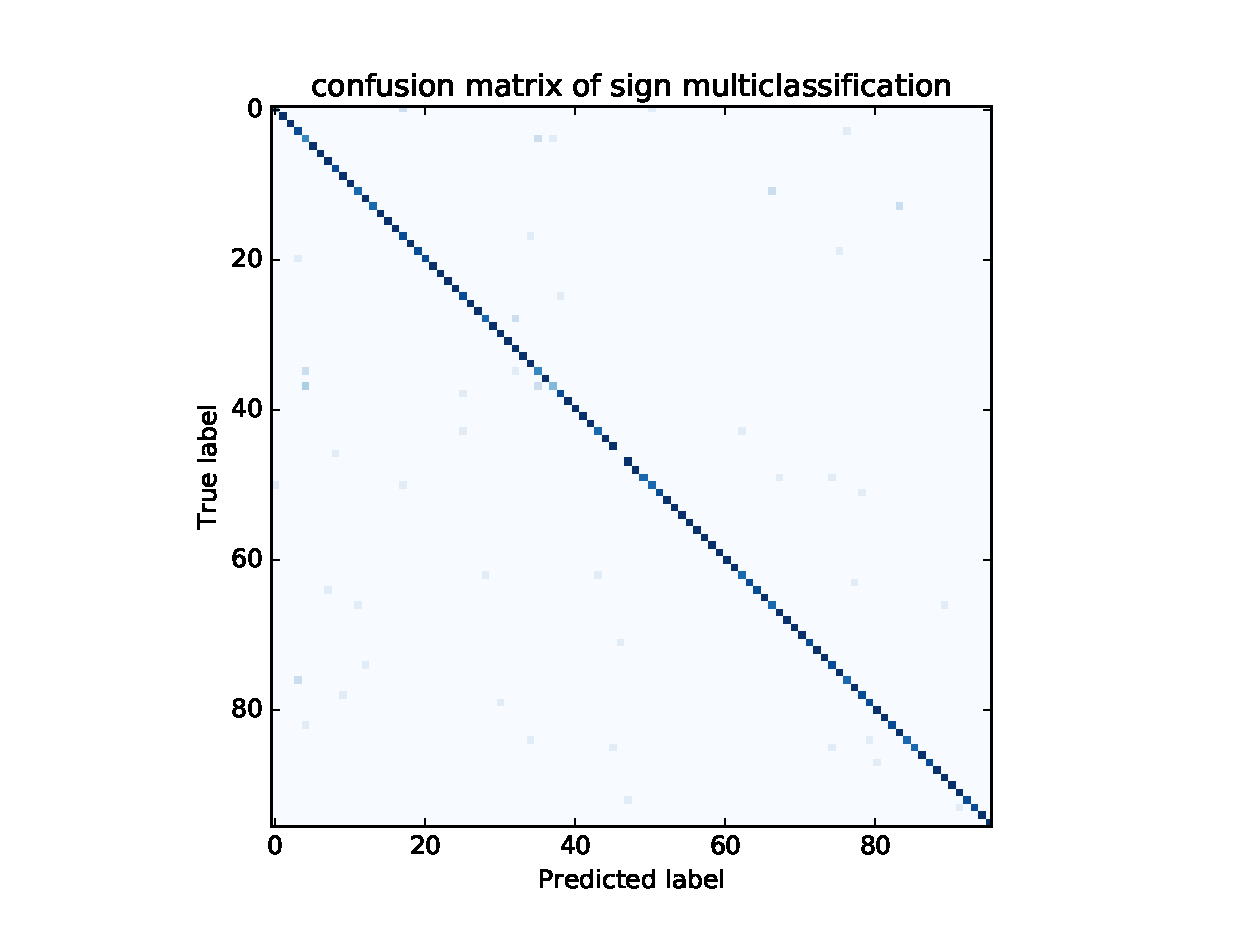
\includegraphics[trim=100 22 80 39, clip,width=1.0\linewidth]{results/svm_high_quality_confusion}
        \caption{High Quality}
\end{subfigure}%
~
\begin{subfigure}[b]{0.48\linewidth}
        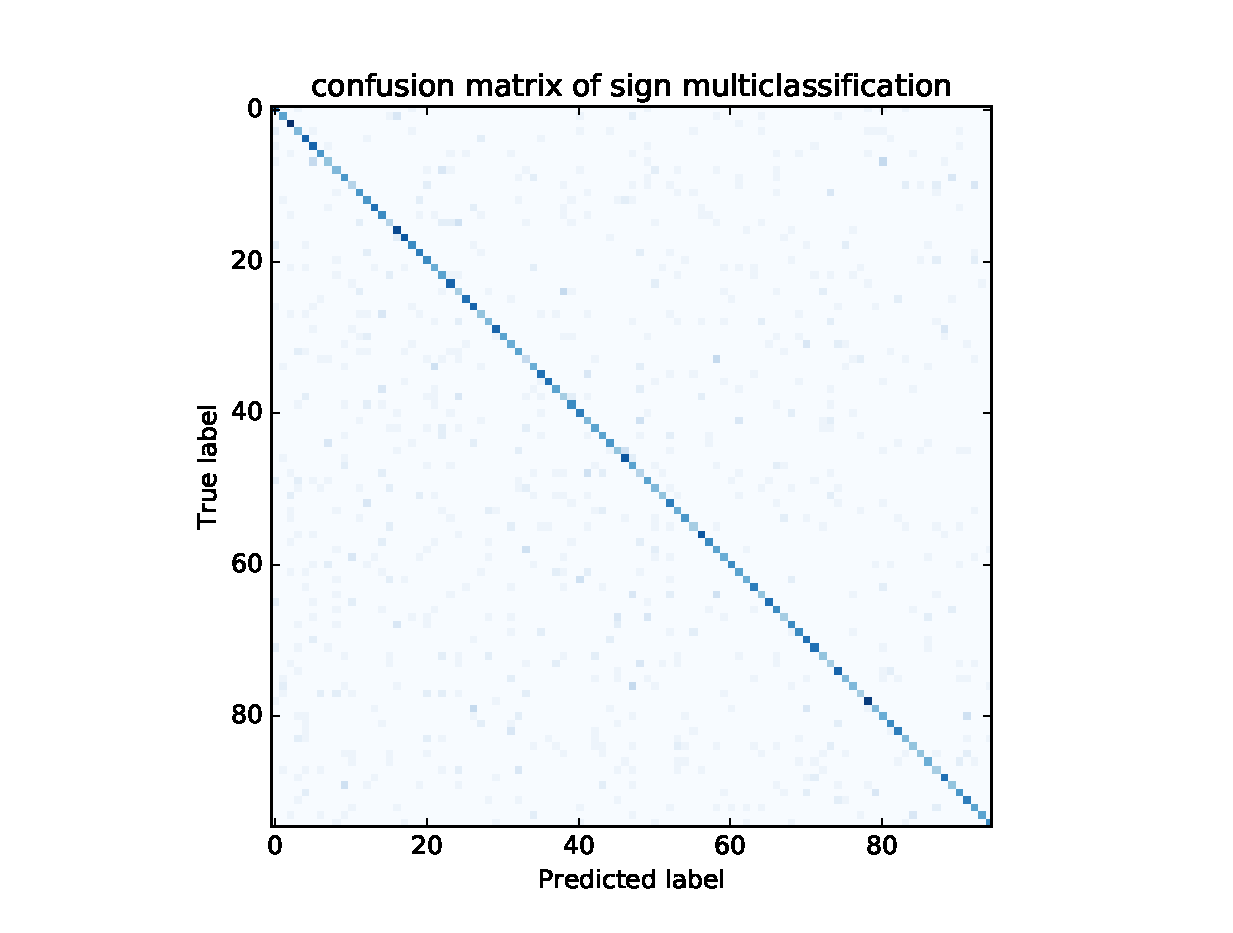
\includegraphics[trim=100 22 80 39, clip,width=1.0\linewidth]{results/svm_low_quality_confusion}
        \caption{Low quality}
\end{subfigure}%
\vspace{-2mm}
\caption{Confusion matrix for SVM}
\label{fig:confusion_matrix_svm}
\end{figure}

Note that the confusion matrix as well as the metrics on the low quality dataset are much worse than those on the high quality dataset. In general, our classifier confused similar signs more often, which is expected because there might not have been enough features to distinguish these signs. Our goal will be to improve performance on lower quality data sets.

Finally, we also tried to perform some analysis on our feature space, to see if it was truly separable in the high dimensional space. We hypothesize that each class has its own cluster in the high dimensional space and is far from other classes. One way to confirm this is to use PCA to reduce the feature space to 3 dimensions and plot the data. We see in Figure \ref{fig:feature_space} that examples from the same class (indicated by similar colors) cluster together, which indicates the presence of the clusters in the higher dimensional space. 

\begin{figure}[h]
    \centering
    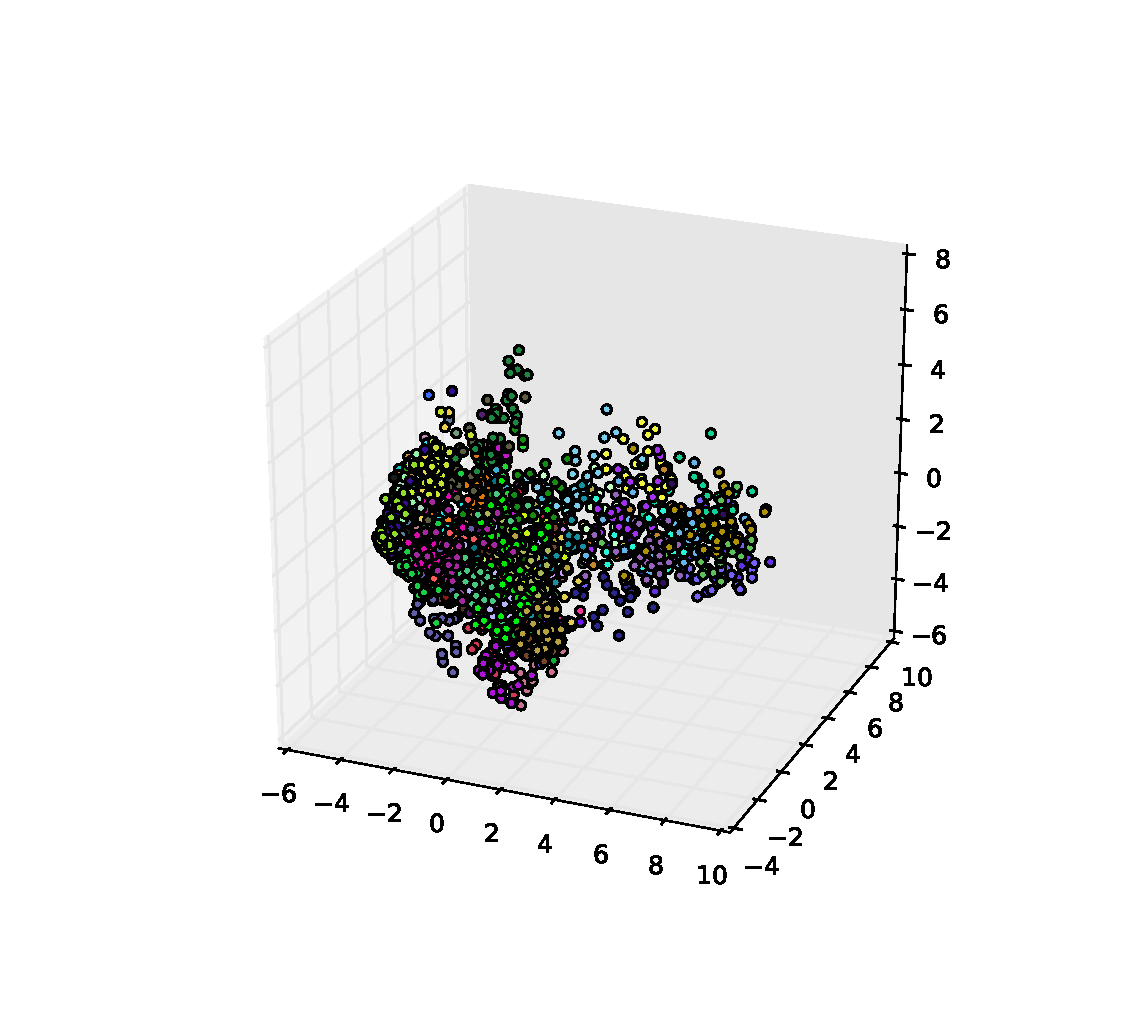
\includegraphics[trim=100 40 80 80, clip, width=0.8\linewidth]{results/feature_space}
    \caption{Feature space reduced to three dimensions}
    \label{fig:feature_space}
\end{figure}

\section{References}
\printbibliography[heading=none]

\section{Appendix}
\begin{figure}[h]
\centering
\begin{subfigure}[b]{0.48\linewidth}
        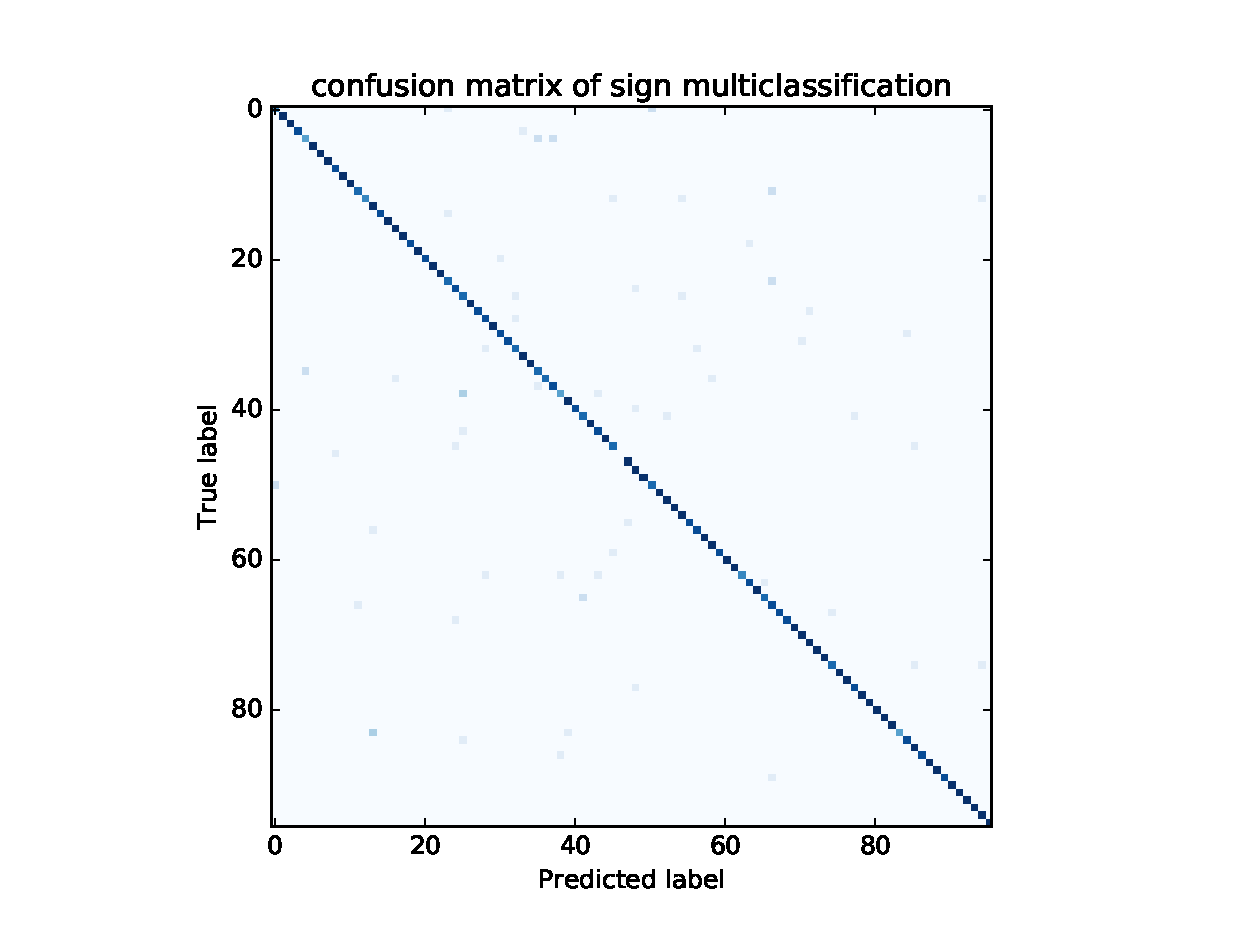
\includegraphics[trim=100 22 80 39, clip,width=1.0\linewidth]{results/logreg_high_quality_confusion}
        \caption{High Quality}
\end{subfigure}%
~
\begin{subfigure}[b]{0.48\linewidth}
        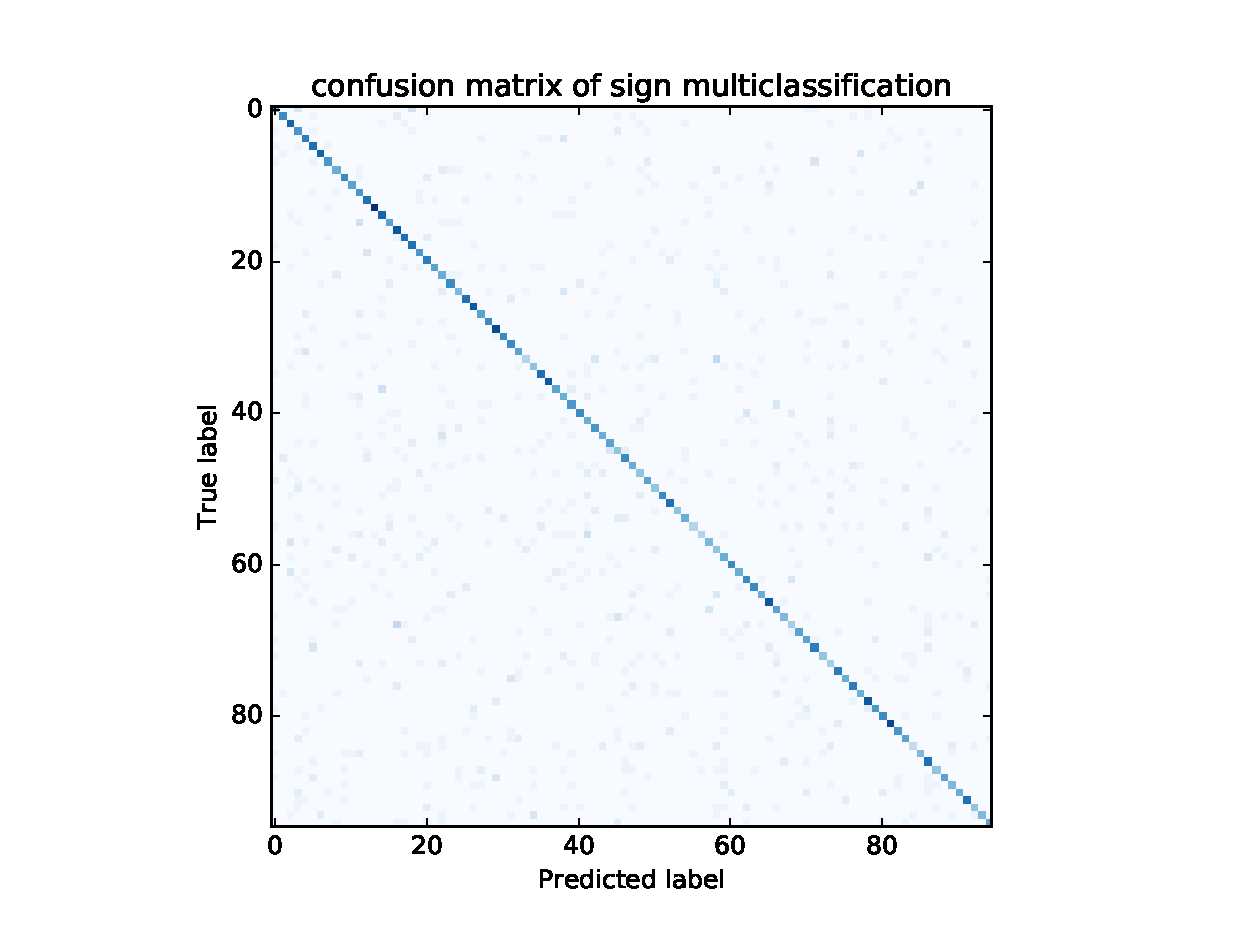
\includegraphics[trim=100 22 80 39, clip,width=1.0\linewidth]{results/logreg_low_quality_confusion}
        \caption{Low quality}
\end{subfigure}%
\vspace{-2mm}
\caption{Confusion matrix for Logistic regression}
\label{fig:confusion_matrix_logreg}
\end{figure}

\end{document}

